%DO NOT MESS AROUND WITH THE CODE ON THIS PAGE UNLESS YOU %REALLY KNOW WHAT YOU ARE DOING
\chapter{Introduction to Kinect Sensor} \label{Introduction to Kinect Sensor}

\section{Kinect v2 Sensor Specifications} \label{Kinect v2 Sensor Specifications}
\noindent Microsoft Kinect Sensor was initially marketed to add motion control to games and is used as a peripheral for Xbox 360. Based on a webcam-style add-on peripheral, it enabled users to control and interact with their console/computer without the need for a game controller, through a natural user interface using gestures and spoken commands.

\begin{figure}[H]
\centering
{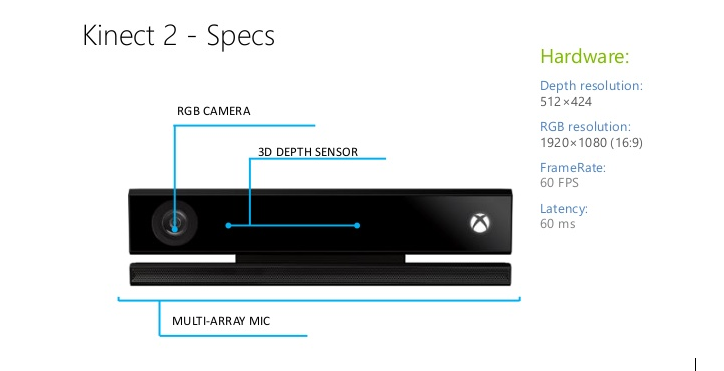
\includegraphics[scale=0.8]{figkinect.png}}
\caption{Microsoft Kinect V2 Sensor}
\end{figure}
\newpage
\noindent The second version of the Kinect that is used in this study was released with Xbox One on November 22, 2013. This new hardware and software provided many improvements, including:

\noindent 1. Improved body tracking - The enhanced fidelity of the depth camera, combined with improvements in the software, have led to a number of body tracking developments. The latest sensor tracks as many as six complete skeletons (compared to two with the V1), and 25 joints per person (compared to 20 with the V1). The tracked positions are more anatomically correct and stable and the range of tracking is broader.

\noindent 2. Improved depth sensing - With higher depth fidelity and a significantly improved noise floor, the sensor gives you improved 3D visualization, improved ability to see smaller objects and all objects more clearly, and improves the stability of body tracking.

\noindent 3. 1080p colour camera (30 Hz, 15 Hz in low light) - The colour camera captures full, beautiful 1080p videos that can be displayed in the same resolution as the viewing screen, allowing for a broad range of powerful scenarios. In addition to improving video communication and video analytic applications, this provides a stable input on which high quality, interactive applications are built.

\noindent 4. New active infrared (IR) capabilities (512 x 424 30 Hz) - In addition to allowing the sensor to see in the dark, the new IR capabilities produce a lighting-independent view—and you can now use IR and colour at the same time.

\noindent 5. The Kinect V2 has a range of 0.5 to 4.5m
\newpage
\def\arraystretch{1.7}
\begin{table} [t]

\begin{tabular}{ |p{5cm}||p{5cm}|p{5cm}| }
 \hline
 \cellcolor{pink} & \cellcolor{pink} Version 1  &  \cellcolor{pink} Version 2 \\
 \hline
Depth Range  & 0.4m to 4m  & 0.5m to 4.5m  \\
Colour Stream & 640x480 @30fps & 1920x1080 @30fps \\
Depth Stream  & 320x240  & 512x424  \\
Infrared Stream & None & 512x424  \\
Type Of Light  & Light Coding  & ToF  \\
Audio Stream & 4-mic array 16khz & 4-mic array 48khz \\
USB  & 2.0  & 3.0  \\
Bodies Tracked  & 2(+4) & 6  \\
Joints & 20 & 25 \\
Hand Tracking & External Tools  & Yes  \\
Face Tracking  & Yes  & Yes+Expressions  \\
FOV & 57$^{\circ}$H 43$^{\circ}$V & 70$^{\circ}$H 60$^{\circ}$V \\
Tilt  & Motorised  & Manual  \\
\hline
\end{tabular}
\caption{Differences between Kinect v1 and v2}
\end{table}

\clearpage


\section{Skeleton Tracking} \label{Skeleton Tracking} 
\noindent By using the depth stream, the Kinect SDK is able to detect the presence of the person in front of the sensor. Kinect is capable of simultaneously tracking upto six people, including two active individuals for gait analysis with a feature extraction of 25 joints per person. The number of people the device can “see” (but not process as individuals) is only limited by how many will fit in the field-of-view of the camera. For each tracked person, Kinect SDK API provides a “skeleton” as a set of motion data. A skeleton contains 25 position sets, one for each “joint” of the body.

\begin{figure}[H]
\centering
{\includegraphics[scale=0.85]{figbodjoints.png}}
\caption{Joints Represented by Skeleton Tracking}
\end{figure}
\newpage

\section{Measuring Distances Using Kinect } \label{ Measuring Distances Using Kinect}             
\noindent Kinect integrates an infrared sensor, along with a depth processor. The visible area is called “field of view”. The depth processor produces depth frames. Each depth frame is a grid of points. The Kinect SDK is then feeding the depth frames to a powerful body-detection algorithm. The algorithm identifies 25 human body joints and calculates their coordinates in the 3D space. 
\noindent Every single joint has 3 values: X, Y, and Z. It is projected in a Cartesian coordinate system. The  point is the position of the sensor. Every other point is measured in terms of the position of the sensor. Check the graph below,It is viewing the sensor and the scene from above.

•	X is the position in the horizontal axis.

•	Y is the position in the vertical axis.

•	Z is the position in the depth axis.


\begin{figure}[H]
\centering
{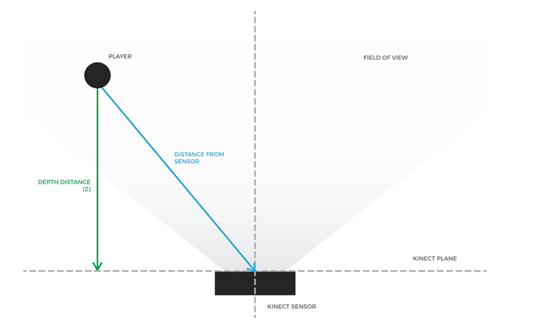
\includegraphics[scale=0.75]{figsensor.png}}
\caption{Measurement of distances using Kinect}
\end{figure}

\noindent As seen from the figure, Z value is not the linear distance between the point and the sensor. Instead, it’s the distance between the point and the plane of the sensor


